\section{数值方法}
\label{sec:numerical}
数学上可以用逆散射方法得到非线性 Schr\"odinger 方程的解析解,也可以用矩方法、变分法得到半解析半近似的解。虽然解析解能很好地反映脉冲在光纤中传输的物理图像,但是大部分实际问题求解析解非常繁琐或是根本就无法用解析方法求解。因此通过数值方法求解非线性 Schr\"odinger 方程来研究光脉冲的非线性传输是必要的。求解这种非线性偏微分方程的数值方法大致可以分为两类
\begin{enumerate}[label=(\arabic*)]
    \item 通过频谱间接求解,分步 Fourier 方法(split-step Fourier method,简称 SSFM)和伪谱方法(pseudospectral method);
    \item 在时域中直接求解,有限差分法(finite difference method,简称 FDM)。
\end{enumerate}
\subsection{伪谱方法}
{\bfseries Fourier 积分变换可以把时域(或空间域)的偏微分方程转换为频域的常微分方程,通过求解频域的常微分方程,再进行逆 Fourier 变换得到偏微分方程的时域(空间域)的解(见图\ref{fig:Fourier_pde})。将此方法应用于偏微分方程离散求解,就是伪谱方法\cite{zhangxiao}。}

要在计算机上实现伪谱方法,有两个问题需要解决
\begin{enumerate}[label=(\arabic*)]
    \item 实现离散数据序列时域与频域的互相转换;
    \item 实现常微分方程的数值求解。
\end{enumerate}
快速 Fourier 变换(fast Fourier transform,简称 FFT)可以很方便地实现离散 Fourier 变换(MATLAB 提供了快速 Fourier 变换的指令 fft 和 ifft);通常用 Runge-Kutta 方法求解常微分方程的数值解(MATLAB 中集成了非常多用 Runge-Kutta 方法设计的 ODE 求解器,比如最常用的 ode45)\cite{Anne}。因此,应用伪谱方法求解偏微分方程在技术上是可行的,求解步骤也十分清楚\cite{zhangxiao}
\begin{enumerate}[label=(\arabic*)]
    \item 对偏微分方程做时域(或空间域)的 Fourier 变换,再将其离散化;
    \item 调用 ODE 求解器对离散化的常微分方程进行求解;
    \item 用 ifft 函数将频域上的计算结果转换为时域(或空间域)上的结果。
\end{enumerate}

1978 年,Fornberg 和 Whitham 提出用伪谱方法求解非线性
Schrödinger 方程\cite{Fornberg}。对于非线性 Schr\"odinger 方程(\ref{eq:NLSE}),通常选择做时域 Fourier 变换,得到脉冲传输(频域)的常微分方程\footnote{应用伪谱方法求解非线性 Schr\"odinger 方程要求脉冲在时域具有周期性,这在光纤传输中是可行的。}
\begin{align}
    &\frac{\partial \widetilde{u}}{\partial \xi}=-\frac{i\omega^2}{2}\widetilde{u}+i\mathscr{F}\left[\left|\mathscr{F}^{-1}[\widetilde{u}]\right|^2\mathscr{F}^{-1}[\widetilde{u}]\right]\\
    &\widetilde{u}(0,\omega)=\mathscr{F}\left[N\cdot\mathrm{sech}(\tau)\right]
\end{align}
将该方程离散化后调用 ode45 指令求解离散后的频域演化方程,再用 ifft 函数将频域结果转换为时域演化过程(详见附录1)。

图\ref{fig:third soliton_time} 和图\ref{fig:third soliton_frequent} 就是用伪谱方法计算输入脉冲 $u(0,\tau)=3\mathrm{sech(\tau)}$ 在光纤中传输得到的三阶光孤子演化结果。用伪谱方法对高阶孤子进行数值模拟,同样得到了脉冲窄化、分裂、再恢复的周期性物理过程(见图\ref{fig:Fourier spectral method})。
\begin{figure}[tbp]
    \centering
    \begin{subfigure}[t]{0.85\linewidth}
        \captionsetup{justification=centering} 
        \begin{minipage}[b]{1\linewidth}
        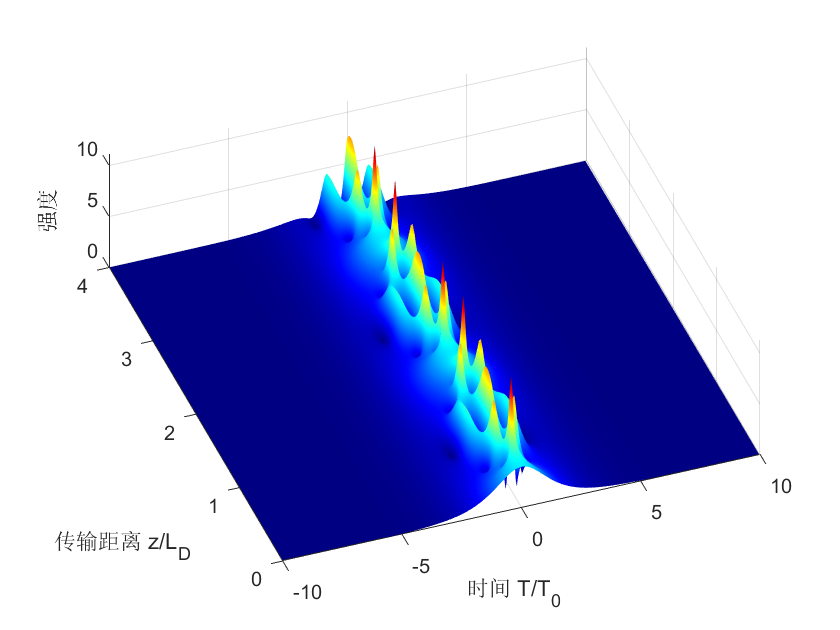
\includegraphics[width=0.45\linewidth]{FSM_四阶孤子演化_侧视图.png}
        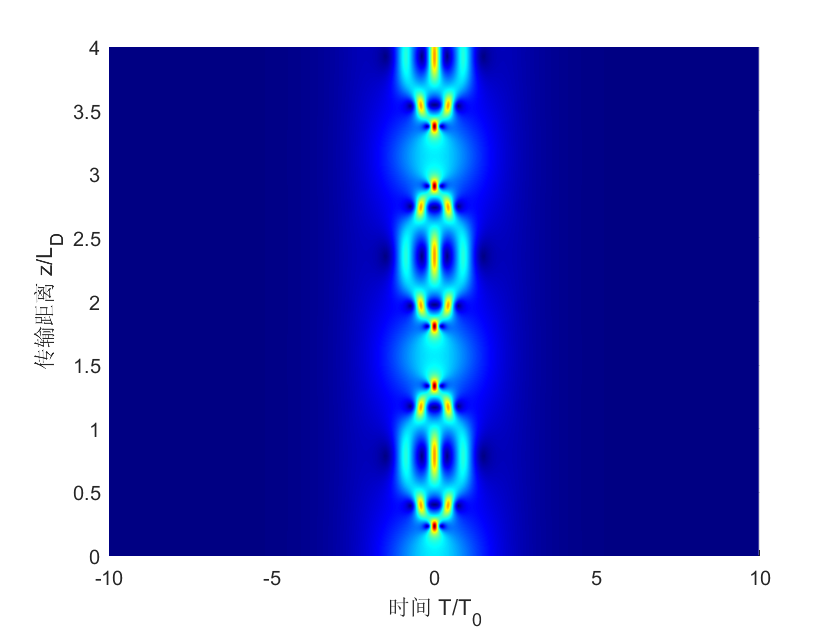
\includegraphics[width=0.45\linewidth]{FSM_四阶孤子演化_俯视图.png}
        \caption{$u(0,\tau)=4\mathrm{sech}(\tau)$}
        \end{minipage}
    \end{subfigure}\\
    \begin{subfigure}[t]{0.85\linewidth}
        \captionsetup{justification=centering} 
        \begin{minipage}[b]{1\linewidth}
        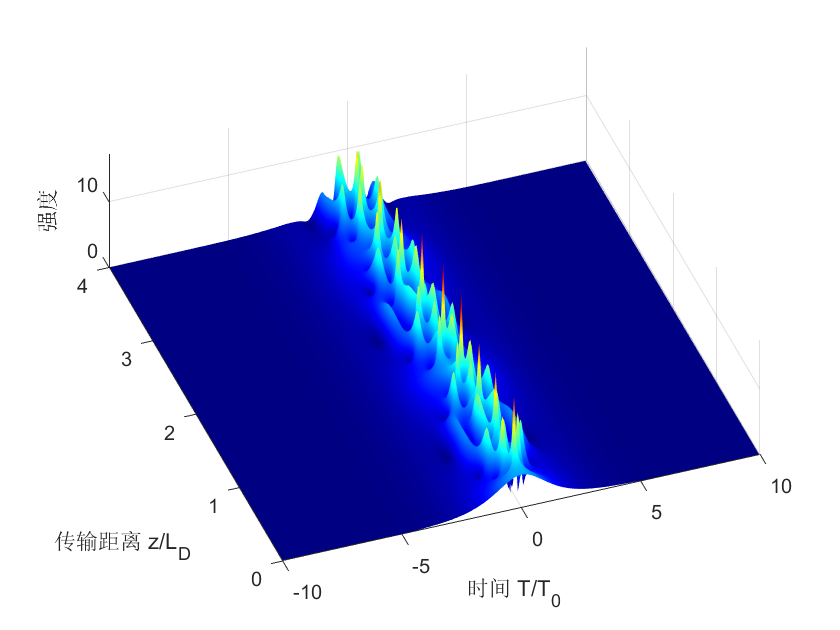
\includegraphics[width=0.45\linewidth]{FSM_五阶孤子演化_侧视图.png}
        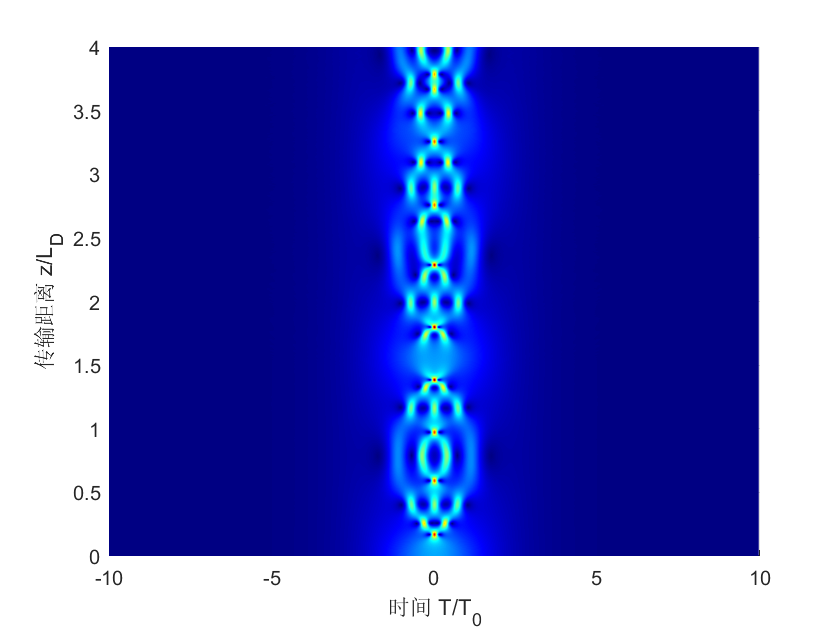
\includegraphics[width=0.45\linewidth]{FSM_五阶孤子演化_俯视图.png}
        \caption{$u(0,\tau)=5\mathrm{sech}(\tau)$}
        \end{minipage}
    \end{subfigure}
    \caption{伪谱方法模拟的高阶孤子周期性演化}
    \label{fig:Fourier spectral method}
\end{figure}
\subsection{分步 Fourier 方法}
伪谱方法在计算机上求解效率高、计算内存小,但是它需要对频域的常微分方程进行数值求解。并且在研究受激 Raman 散射和 受激 Brillouin 散射问题时,需要在非线性 Schr\"odinger 方程中引入高阶色散项和非线性项,这种情形下需要对频域的常微分方程进行降阶等一系列处理,伪谱方法的可拓展性就非常有限。其实早在伪谱方法之前,人们在求解 KdV 方程的时候就应用了分步 Fourier 方法\cite{Tappert,Chellappan},后来这一数值方法被推广到非线性 Schr\"odinger 方程及其他非线性偏微分方程的求解。
\subsubsection{交替计算}
脉冲在光纤中传输时,光场包络同时受色散和非线性效应的影响
\begin{align}
    \frac{\partial A}{\partial z}&=\left(\hat{D}+\hat{N}\right)A \\
    \hat{D}&=-\frac{\alpha}{2}-\frac{i\beta_2}{2}\frac{\partial^2}{\partial T^2}+\cdots \nonumber \\
    \hat{N}&=i\gamma|A|^2+\cdots \nonumber
\end{align}
也就是说,色散效应(线性微分算子 $\hat{D}$)和非线性效应(非线性函数 $\hat{N}$)对包络函数 $A$ 的作用是同步的。分步 Fourier 方法假设光场传输过程中这两种作用交替进行,分别考虑其影响。这种假设从计算结果上看是可行的,能得到光波传输的近似结果\cite{Agrawal,Fisher}。

脉冲从 $z$ 到 $z+h$ 传播一小段距离,这一小段传输过程可以分两步进行:第一步,仅考虑非线性效应的影响,忽略线性算子的作用,$\hat{D}=0$;第二步,仅考虑色散效应的作用,忽略非线性函数的影响,$\hat{N}=0$
\begin{equation}
    A(z+h,T)\approx\exp(h\hat{D})\exp(h\hat{N})A(z,T)
\end{equation}
非线性效应的影响 $\exp(h\hat{N})$ 可以在时域中计算,色散效应的影响 $\exp(h\hat{D})$ 在频域中计算更为方便
\begin{equation}
    \exp(h\hat{D})B(z,T)=\mathscr{F}^{-1}\left[\exp(h\hat{D}(-i\omega))\mathscr{F}[B(z,T)]\right]
\end{equation}
其中,$\hat{D}(-i\omega)$ 表示用 $-i\omega$ 去替换时域微分算子 $\partial/\partial T$\cite{Agrawal}。

最原始的分步 Fourier 方法是非常不精确的,因为它忽略了算子 $\hat{D}$ 和算子 $\hat{N}$ 的非对易性,根据 Baker-Campbell-Hausdorf(BCH)公式
\begin{equation}
    \exp(\hat{a})\exp(\hat{b})=\exp\left(\hat{a}+\hat{b}+\frac{1}{2}[\hat{a},\hat{b}]+\frac{1}{12}[\hat{a}-\hat{b},[\hat{a},\hat{b}]]+\cdots\right)
\end{equation}
可知对易子 $h^2[\hat{D},\hat{N}]$ 是分步 Fourier 方法误差的主要来源,因此分步 Fourier 方法产生的空间截断误差是 $O(h^2)$。
\subsubsection{改进分步 Fourier 方法}
可以对脉冲在 $z$ 到 $z+h$ 小区间上传输过程做不同的假设,以提高分步 Fourier 方法的精度。比较常用的一种方案是对称分步 Fourier 方法,该方法假定非线性效应作用在每个小区间的中间
\begin{equation}
    A(z+h,T)\approx\exp\left(\frac{h}{2}\hat{D}\right)\exp\left(\int_z^{z+h}\hat{N}(z')\mathrm{d}z'\right)\exp\left(\frac{h}{2}\hat{D}\right)A(z,T)
    \label{eq:SSFM}
\end{equation}
{\bfseries 分步 Fourier 方法的物理过程是非常直观的(见图\ref{fig:SSFM})。脉冲 $A(z,T)$ 在最初的 $h/2$ 距离上传输时仅考虑色散作用;在 $z+h/2$ 的处,包络乘以非线性的积分项,表示整个小区间上的非线性效应;脉冲在剩下的 $h/2$ 距离上的传输也只与色散有关,最终得到 $A(z+h,T)$\cite{Agrawal}。}
\begin{figure}[btp]
    \centering
    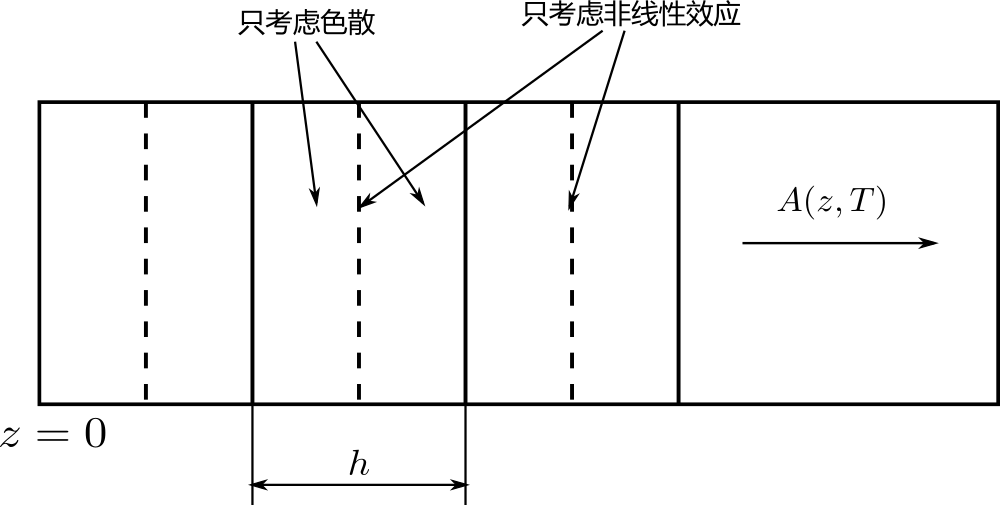
\includegraphics[width=0.5\textwidth]{SSFM.png}
    \caption{分步 Fourier 方法示意图}
    \label{fig:SSFM}
\end{figure}

应用 BCH 公式可知对称分步 Fourier 方法的主要误差来自双对易子 $h^3[\hat{N},[\hat{D},\hat{N}]]$ 和 $h^3[\hat{D},[\hat{D},\hat{N}]]$,因此分步 Fourier 方法的截断误差 $O(h^3)$。

分步 Fourier 方法很容易在计算机上实现。可将长度为 $L$ 的光纤划分为 $M$ 个计算区间,若步长 $h=L/M$ 足够小,包含非线性算子积分的指数项可以近似为 $\exp(h\hat{N})$。应用(\ref{eq:SSFM})给出的传输假设
\begin{equation}
    A(L,T)\approx e^{-\frac{1}{2}h\hat{D}}\left(\prod_{m=1}^Me^{h\hat{D}}e^{h\hat{N}}\right)e^{\frac{1}{2}h\hat{D}}A(0,T)
\end{equation}
当然也可以把色散作用集中在每一个小区间的中间,得到另一种不同的算法
\begin{equation}
    A(L,T)\approx e^{-\frac{1}{2}h\hat{N}}\left(\prod_{m=1}^Me^{h\hat{N}}e^{h\hat{D}}\right)e^{\frac{1}{2}h\hat{N}}A(0,T)
    \label{eq:1/2N->D->1/2N}
\end{equation}

图\ref{fig:SSFM_second_soliton} 给出了用对称分步 Fourier 方法(\ref{eq:1/2N->D->1/2N})实现的二阶孤子的时域和频域演化过程(计算代码详见附录2);图\ref{fig:FSM_second_soliton} 给出的是相同步长 $h$ 下伪谱方法计算所得的结果。将其与二阶孤子解析结果(见图\ref{fig:second soliton})进行对比发现
\begin{enumerate}[label=(\arabic*)]
    \item 伪谱方法脉冲传输的计算结果与解析解非常吻合;而分步 Fourier 方法却不能很好地体现孤子周期性,并且随着传输距离的增加,计算结果会在在脉冲的前沿和后沿出现振荡;
    \item 从频域结果看,伪谱方法所得频谱可以体现自相位调制和反常色散交替影响的结果;而分步 Fourier 方法所得结果中出现了频移的小峰,这部分较小的频移导致脉冲边缘在传输过程中的振荡。
\end{enumerate}
\begin{figure}[tbp]
    \centering
    \begin{subfigure}[t]{0.85\linewidth}
        \captionsetup{justification=centering} 
        \begin{minipage}[b]{1\linewidth}
        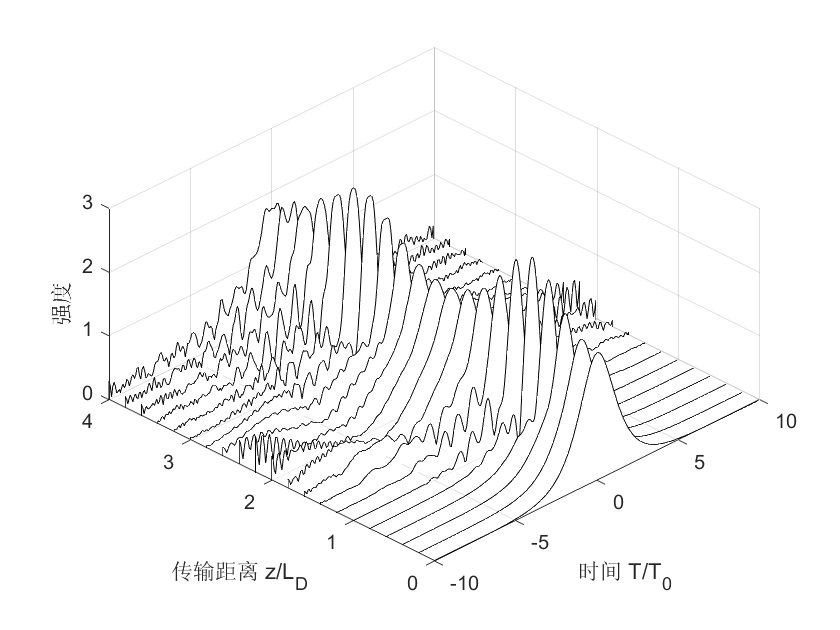
\includegraphics[width=0.45\linewidth]{SSFM_二阶孤子_时域.png}
        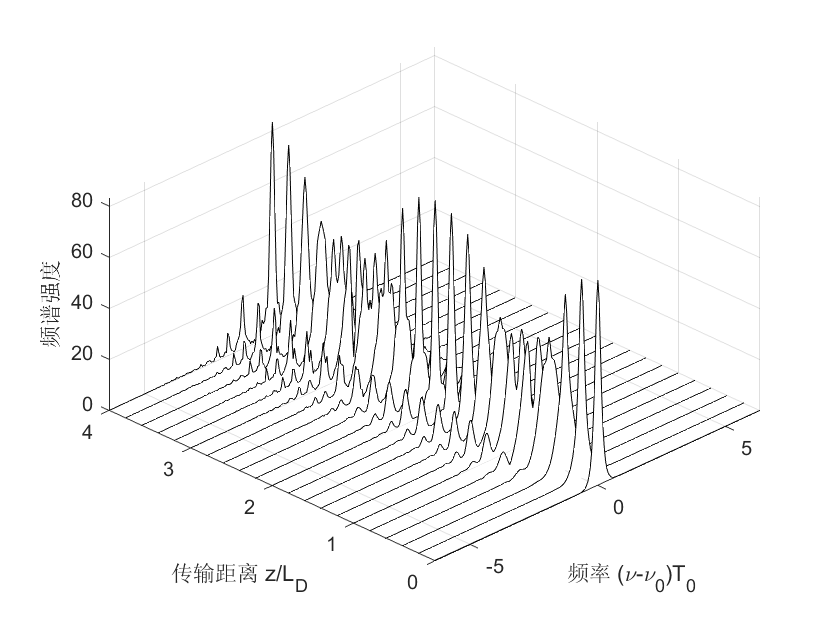
\includegraphics[width=0.45\linewidth]{SSFM_二阶孤子_频域.png}
        \caption{分步 Fourier 方法求解孤子时域演化和频谱($h=0.2$)}
        \label{fig:SSFM_second_soliton}
        \end{minipage}
    \end{subfigure}\\
    \begin{subfigure}[t]{0.85\linewidth}
        \captionsetup{justification=centering} 
        \begin{minipage}[b]{1\linewidth}
        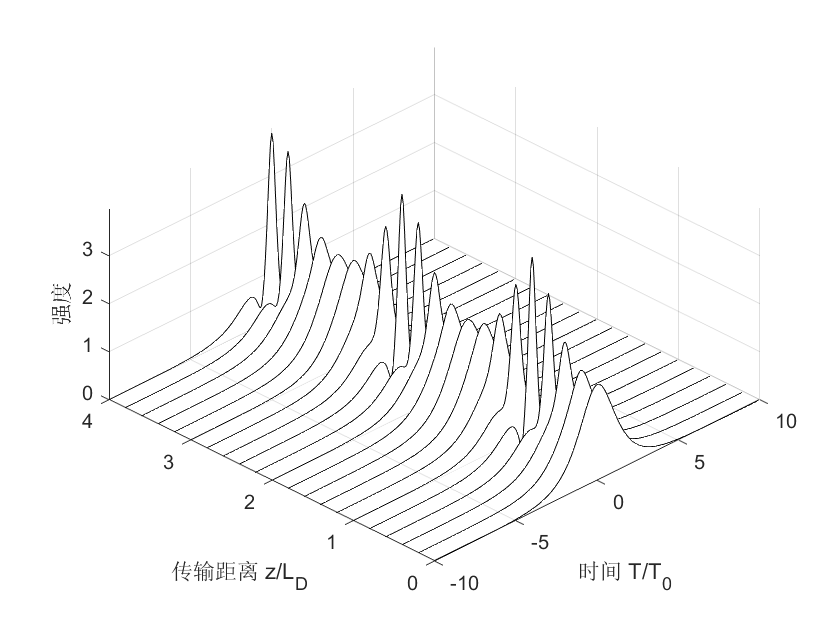
\includegraphics[width=0.45\linewidth]{FSM_二阶孤子_时域.png}
        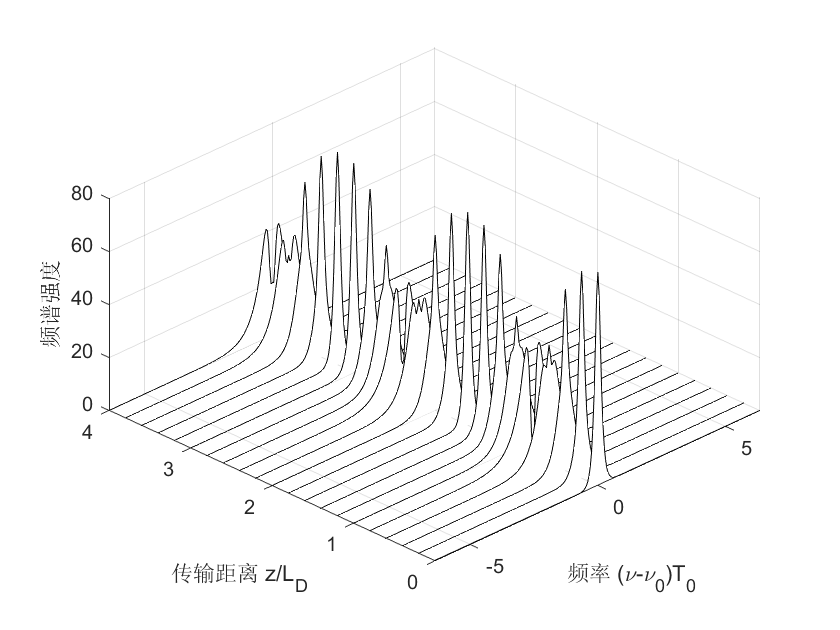
\includegraphics[width=0.45\linewidth]{FSM_二阶孤子_频域.png}
        \caption{伪谱方法求解孤子时域演化和频谱($h=0.2$)}
        \label{fig:FSM_second_soliton}
        \end{minipage}
    \end{subfigure}
    \caption{分步 Fourier 方法和伪谱方法求解二阶孤子结果对比}
\end{figure}
导致分步 Fourier 方法计算结果不准确的主要原因是用 $\exp(h\hat{N})$ 代替了非线性算子积分的指数项进行求解。可用迭代的方法计算近似积分,过程比较繁琐,但是通过减小区间步长 $h$ 一样可以得到更可靠的结果。因此,采用更小的空间步长计算,分步 Fourier 方法可以得到和伪谱方法类似的求解结果(见图\ref{fig:split-step Fourier method})。
\begin{figure}[tbp]
    \centering
    \begin{subfigure}[t]{0.85\linewidth}
        \captionsetup{justification=centering} 
        \begin{minipage}[b]{1\linewidth}
        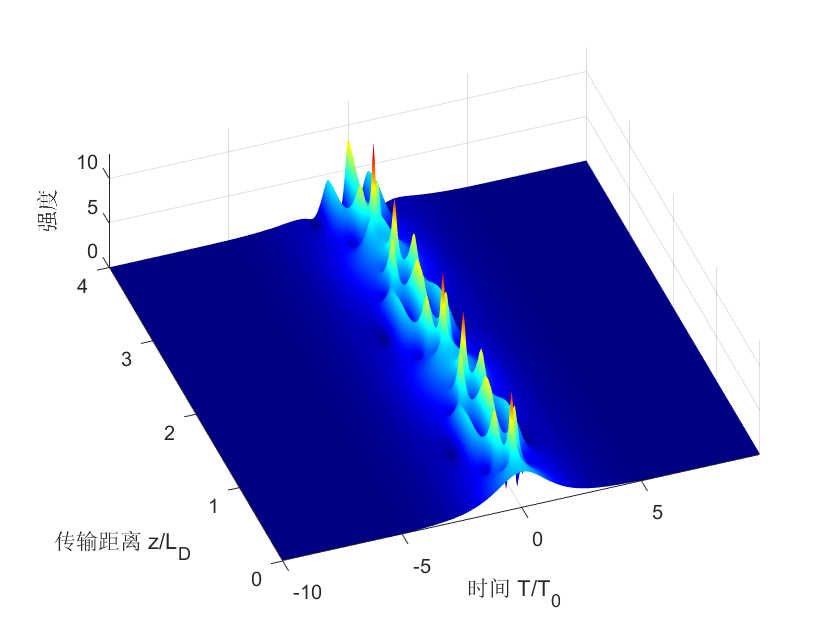
\includegraphics[width=0.45\linewidth]{SSFM_四阶孤子_侧视图.png}
        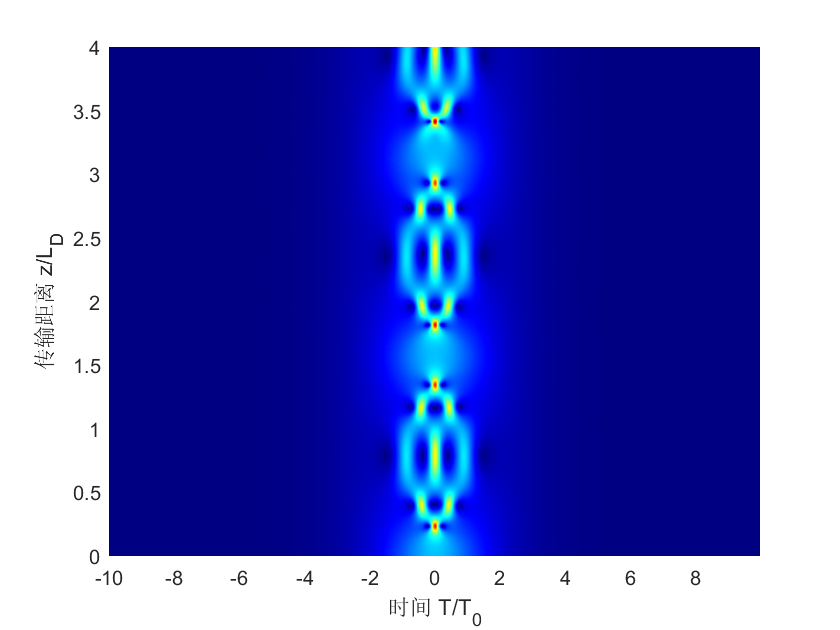
\includegraphics[width=0.45\linewidth]{SSFM_四阶孤子_俯视图.png}
        \caption{$u(0,\tau)=4\mathrm{sech}(\tau)$}
        \end{minipage}
    \end{subfigure}\\
    \begin{subfigure}[t]{0.85\linewidth}
        \captionsetup{justification=centering} 
        \begin{minipage}[b]{1\linewidth}
        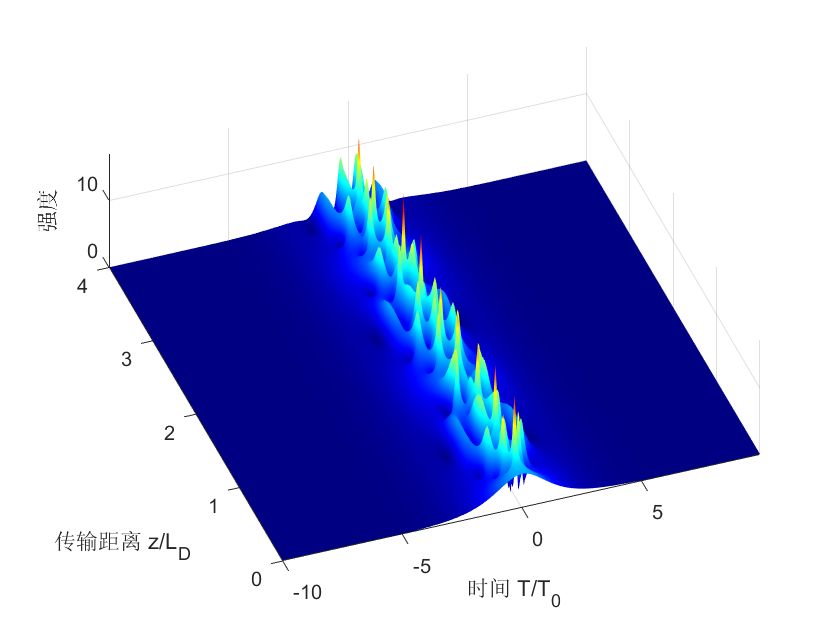
\includegraphics[width=0.45\linewidth]{SSFM_五阶孤子_侧视图.png}
        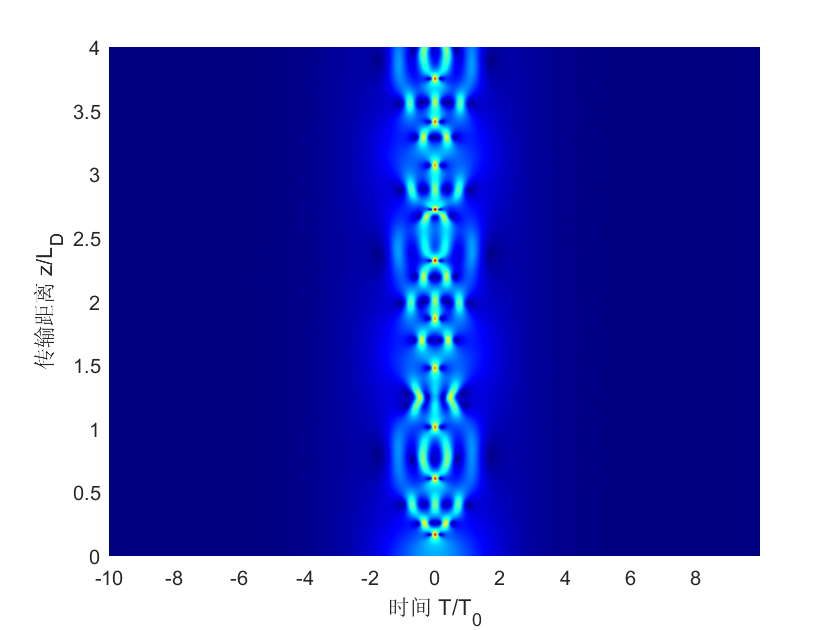
\includegraphics[width=0.45\linewidth]{SSFM_五阶孤子_俯视图.png}
        \caption{$u(0,\tau)=5\mathrm{sech}(\tau)$}
        \end{minipage}
    \end{subfigure}
    \caption{分步 Fourier 方法模拟的高阶孤子周期性演化}
    \label{fig:split-step Fourier method}
\end{figure}

\subsection{有限差分法}
{\bfseries 有限差分法是人们在研究微分方程时发展起来的一种数值技术,该方法的基本思想是用差分近似代替微分方程中的微分,把复杂的微分方程问题转化为计算机上容易处理的差分方程(代数方程)问题。利用有限差分法求解偏微分方程基本包括三个步骤\cite{yangbojun}
\begin{enumerate}[label=(\arabic*)]
    \item 将求解区域离散化(划分网格节点);
    \item 对偏微分方程和定解条件做差分近似(构造差分格式);
    \item 求解差分方程组(一般采用迭代法求解)。
\end{enumerate}}

首先,对非线性 Schr\"odinger 方程(\ref{eq:NLSE})的求解区域处理为离散的节点网格
\begin{align}
    u_{n}^{m}&=u(m\Delta\xi,n\Delta\tau)\\
    m&=0,1,2,\cdots,M \nonumber \\
    n&=-N,-N+1,\cdots,-1,0,1,\cdots,N-1,N \nonumber    
\end{align}
其中,上标 $m$ 标记传输距离,下标 $n$ 标记群速度坐标系下的时间。

其次,将非线性 Schr\"odinger 方程近似处理为等效的差分方程。一般应用 Taylor 级数对偏微分方程进行差分近似,比如 Euler 格式、蛙跳(hopscotch)格式、Crank-Nicolson 格式\cite{Taha,Qianshun}。1976 年,Ablowite 和 Ladik 基于逆散射方法提出了针对非线性偏微分方程求解的差分格式\cite{Taha}。

本文仅介绍常用的差分格式,最典型的差分近似是 Euler 差分格式
\begin{equation}
    i\frac{u_n^{m+1}-u_n^{m-1}}{2\Delta \xi}+\frac{u_{n+1}^{m}-2u_n^m+u_{n-1}^m}{2(\Delta\tau)^2}+|u_n^m|u_n^m=0
\end{equation}
Euler 格式是显式差分格式,一阶偏导 $\partial u/\partial \xi$ 为中心差分,二阶偏导 $\partial^2 u/\partial \tau^2$ 也是中心差分,因此其截断误差为 $O((\Delta\xi)^2)+O((\Delta\tau)^2)$。该差分格式的稳定性受 CFL 条件\footnote{该稳定性条件由 Courant、Friedrichs、Lewy 提出,可用 von Neumann 方法推导。}约束
\begin{equation}
    \lambda=\frac{\Delta\xi}{2(\Delta\tau)^2}\leqslant\frac{1}{4}
\end{equation}
当然也可以对非线性项做(时间)平均近似得到蛙跳格式
\begin{subequations}
    \begin{equation}
        i\frac{u_n^{m+1}-u_n^{m}}{\Delta\xi}+\frac{u_{n+1}^m-2u_n^m+u_{n-1}^m}{2(\Delta\tau)^2}+\frac{1}{2}\left(|u_{n+1}^m|^2u_{n+1}^m+|u_{n-1}^m|^2u_{n-1}^m\right)=0
        \label{eq:Hopscotch_explicit}
    \end{equation}
    \begin{equation}
        i\frac{u_n^{m+1}-u_n^{m}}{\Delta\xi}+\frac{u_{n+1}^{m+1}-2u_n^{m+1}+u_{n-1}^{m+1}}{2(\Delta\tau)^2}+\frac{1}{2}\left(|u_{n+1}^{m+1}|^2u_{n+1}^{m+1}+|u_{n-1}^{m+1}|^2u_{n-1}^{m+1}\right)=0
        \label{eq:Hopscotch_implicit}
    \end{equation}
\end{subequations}
把隐式差分格式(\ref{eq:Hopscotch_implicit})的上标 $m$ 代换为 $m-1$,并结合显式差分格式(\ref{eq:Hopscotch_explicit})可以发现蛙跳格式隐含了空间平均的近似
\begin{equation}
    u_n^{m+1}+u_n^{m-1}=2u_n^m
\end{equation}
因此,蛙跳格式的一阶偏导 $\partial u/\partial \xi$ 虽然是前向差分,但是其截断误差也是 $O((\Delta\xi)^2)+O((\Delta\tau)^2)$,并且无条件稳定。

比较常用的是一种差分近似是 Crank-Nicolson 格式,它将二阶偏导项 $\partial^2 u/\partial \tau^2$ 做了平均处理\cite{Greig,Taha}
\begin{equation}
    \begin{aligned}
        i\frac{u_n^{m+1}-u_n^m}{\Delta\xi}&+\frac{1}{4(\Delta\tau)^2}\left[u_{n+1}^{m+1}-2u_n^{m+1}+u_{n-1}^{m+1}+u_{n+1}^{m}-2u_n^{m}+u_{n-1}^{m}\right]\\
        &+\frac{1}{2}\left(|u_{n+1}^m|^2u_{n+1}^m+|u_{n-1}^m|^2u_{n-1}^m\right)=0
    \end{aligned}
\end{equation}
该种差分格式的截断误差为 $O(\Delta\xi)+O((\Delta\tau)^2)$,并且无条件稳定。若要减小 Crank-Nicolson 格式的空间截断误差,可对非线性项做(空间)平均
\begin{equation}
    \begin{aligned}
        i\frac{u_n^{m+1}-u_n^m}{\Delta\xi}&+\frac{1}{4(\Delta\tau)^2}\left[u_{n+1}^{m+1}-2u_n^{m+1}+u_{n-1}^{m+1}+u_{n+1}^{m}-2u_n^{m}+u_{n-1}^{m}\right]\\
        &+\frac{1}{2}\left(|u_n^{m+1}|^2u_n^{m+1}+|u_n^m|^2u_n^m\right)=0
    \end{aligned}
    \label{eq:Crank-Nicolson}
\end{equation}

为了更方便地在计算机上实现差分求解,通常把差分方程改写成矩阵方程的形式,比如对 Crank-Nicolson 格式的差分方程(\ref{eq:Crank-Nicolson}),可用矩阵方程表达\cite{Taha}
\begin{equation}
    \textbf{\textit{A}}\textbf{\textit{u}}^{m+1}=\textbf{\textit{F}}
    \label{eq:matrix}
\end{equation}
其中,差分矩阵 $\textbf{\textit{A}}$ 通常是一个带状矩阵,在周期性边界条件($u_{-N-1}^m=u_N^m$,$u_{N+1}^m=u_{-N}^m$)的假设下
\begin{subequations}
    \begin{equation}
        \textbf{\textit{A}}=\begin{bmatrix}
            i-\lambda & \lambda/2 & & & \lambda/2\\
            \lambda/2 & i-\lambda &\lambda/2 & &\\
             & \ddots & \ddots & \ddots & \\
             & & \lambda/2 & i-\lambda & \lambda/2\\
             \lambda/2 & & & \lambda/2 & i-\lambda
        \end{bmatrix}\hspace{4ex}\textbf{\textit{u}}^{m+1}=\begin{bmatrix}
            u_{-N}\\
            u_{-N+1}\\
            \vdots\\
            u_{N-1}\\
            u_{N}
        \end{bmatrix}^{m+1}
    \end{equation}
    \begin{equation}
        \begin{aligned}
            F_n&=-\frac{\lambda}{2}\left(u_{n+1}^m+u_{n-1}^m\right)+(\lambda+i)u_n^m+\frac{\Delta\xi}{2}\left(|u_n^{m+1}|^2u_n^{m+1}+|u_n^m|^2u_n^m\right)\\
            &\approx-\frac{\lambda}{2}\left(u_{n+1}^m+u_{n-1}^m\right)+(\lambda+i)u_n^m+\Delta\xi|u_n^m|^2u_n^m                
        \end{aligned}
    \end{equation}
\end{subequations}

最后便是求解矩阵方程(\ref{eq:matrix})。差分矩阵 $\textbf{\textit{A}}$ 通常是大型矩阵,用 Gauss 消元法求解矩阵方程(\ref{eq:matrix})会花费较多的计算时间。一般应用迭代方法求解矩阵方程,常用的迭代算法有 Jacobi 迭代、Gauss-Seidel 迭代和逐次超松弛迭代(successive overrelaxation,简称 SOR)方法\cite{Anne},本文不做具体介绍。在 MATLAB 中,应用 spdiags 函数可以很方便地创建差分矩阵 $\textbf{\textit{A}}$,并且 inv 函数可以直接求解带状矩阵 $\textbf{\textit{A}}$ 的逆矩阵,使得有限差分的编程更容易实现(详见附录3)。

有限差分法可以实现单光孤子周期性演化的计算,但是有限差分法耗时非常多,且不容易控制传输距离,很容易产生发散的结果(见图\ref{fig:FDM})。一般情况下,分步 Fourier 方法比有限差分法快一到两个数量级,但是在波分复用系统的计算中,有限差分法比分步 Fourier 方法所用时间更少\cite{Agrawal}。
\begin{figure}[tbp]
    \centering
    \begin{subfigure}[t]{0.85\linewidth}
        \captionsetup{justification=centering} 
        \begin{minipage}[b]{1\linewidth}
        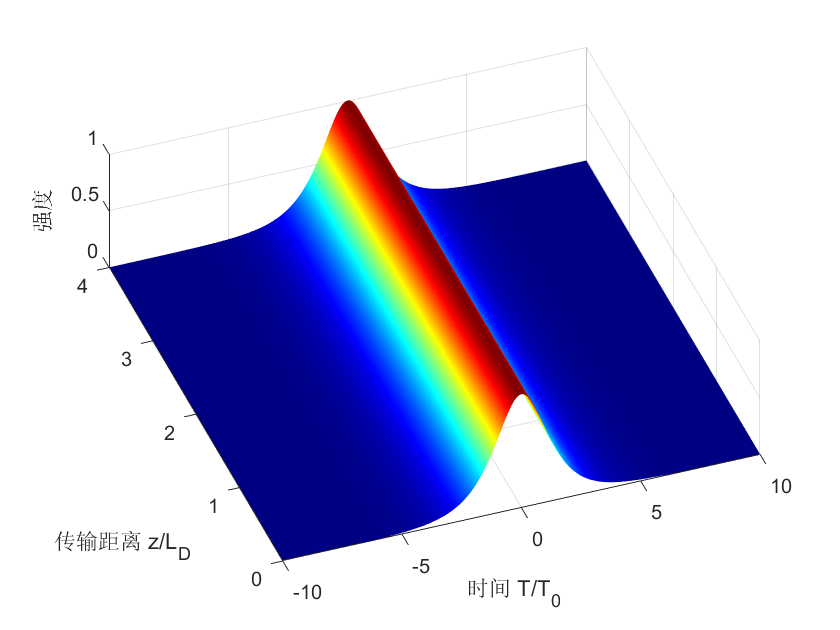
\includegraphics[width=0.45\linewidth]{FDM_基阶孤子_侧视图.png}
        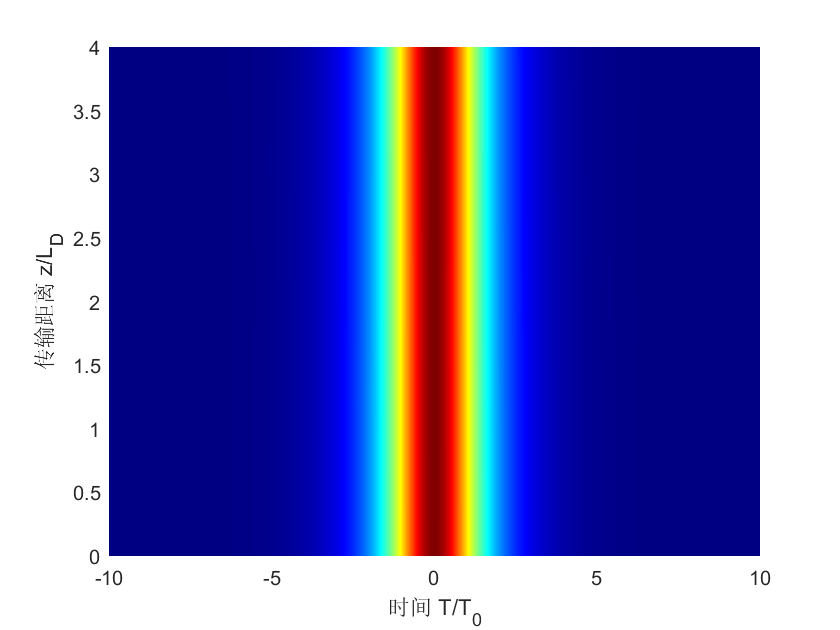
\includegraphics[width=0.45\linewidth]{FDM_基阶孤子_俯视图.png}
        \caption{$u(0,\tau)=\mathrm{sech}(\tau)$}
        \end{minipage}
    \end{subfigure}\\
    \begin{subfigure}[t]{0.85\linewidth}
        \captionsetup{justification=centering} 
        \begin{minipage}[b]{1\linewidth}
        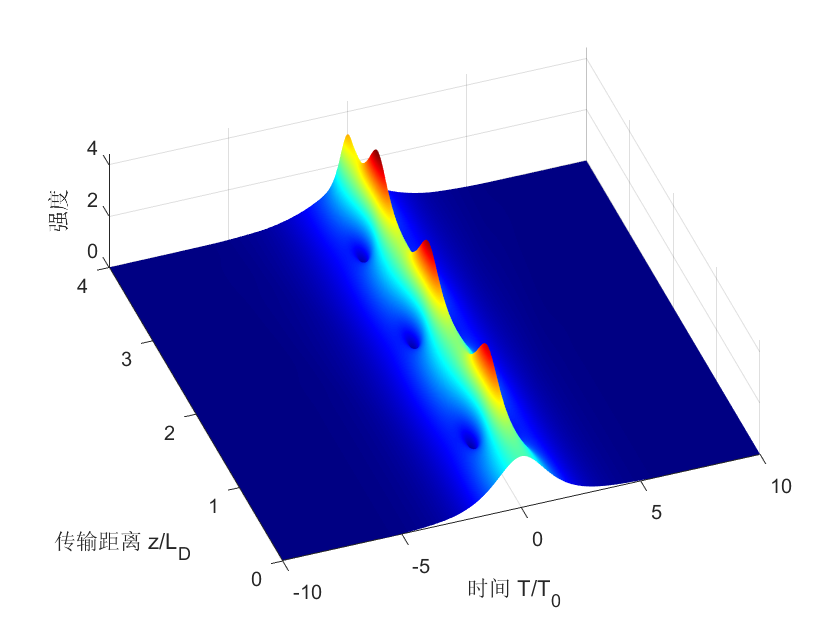
\includegraphics[width=0.45\linewidth]{FDM_二阶孤子_侧视图.png}
        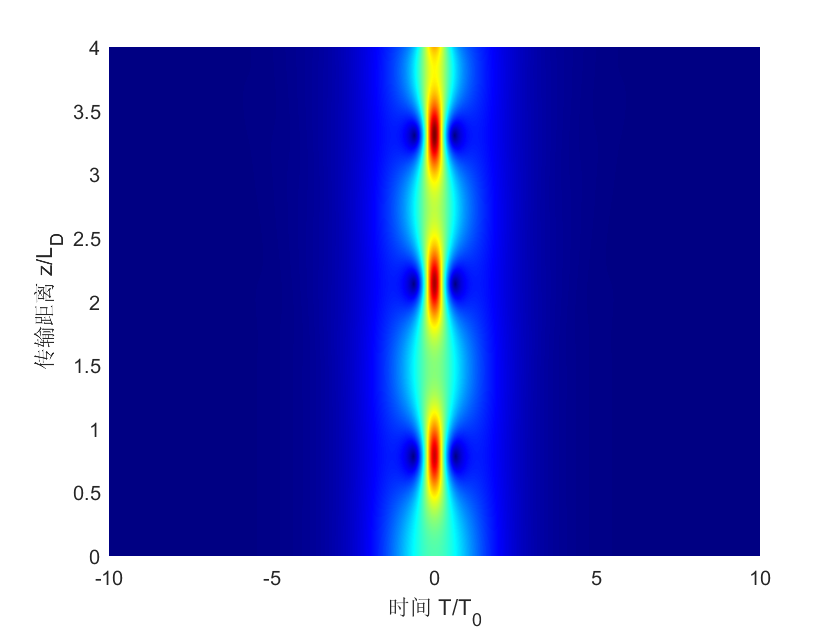
\includegraphics[width=0.45\linewidth]{FDM_二阶孤子_俯视图.png}
        \caption{$u(0,\tau)=2\mathrm{sech}(\tau)$}
        \end{minipage}
    \end{subfigure}\\
    \begin{subfigure}[t]{0.85\linewidth}
        \captionsetup{justification=centering} 
        \begin{minipage}[b]{1\linewidth}
        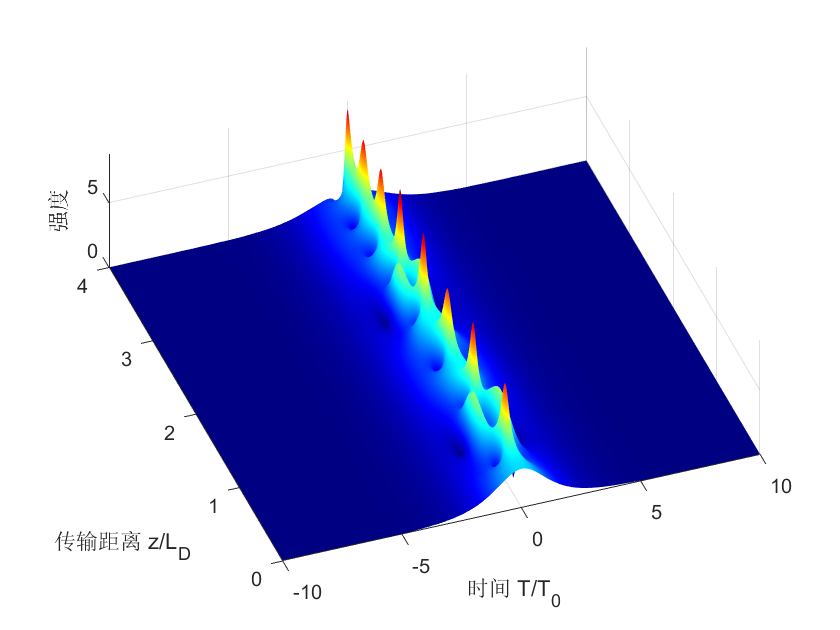
\includegraphics[width=0.45\linewidth]{FDM_三阶孤子_侧视图.png}
        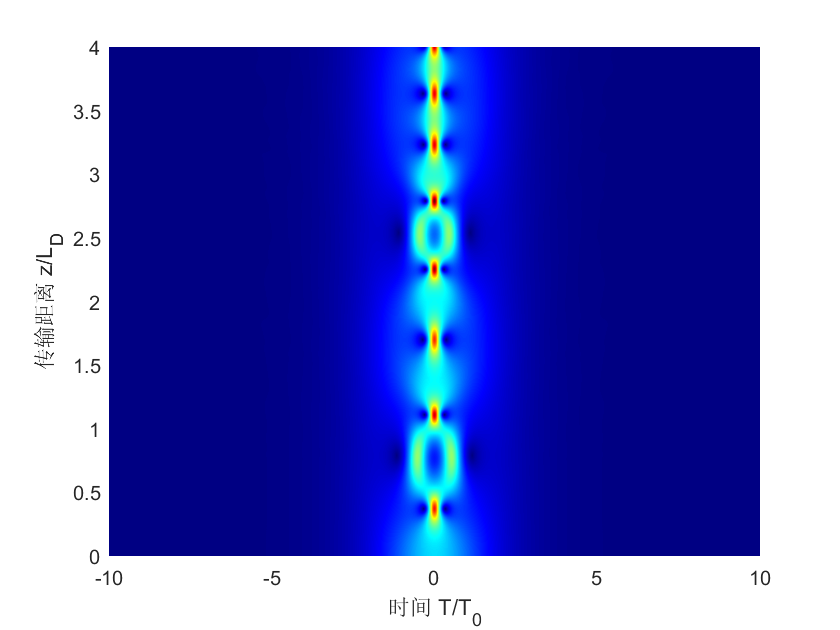
\includegraphics[width=0.45\linewidth]{FDM_三阶孤子_俯视图.png}
        \caption{$u(0,\tau)=3\mathrm{sech}(\tau)$}
        \end{minipage}
    \end{subfigure}\\
    \begin{subfigure}[t]{0.85\linewidth}
        \captionsetup{justification=centering} 
        \begin{minipage}[b]{1\linewidth}
        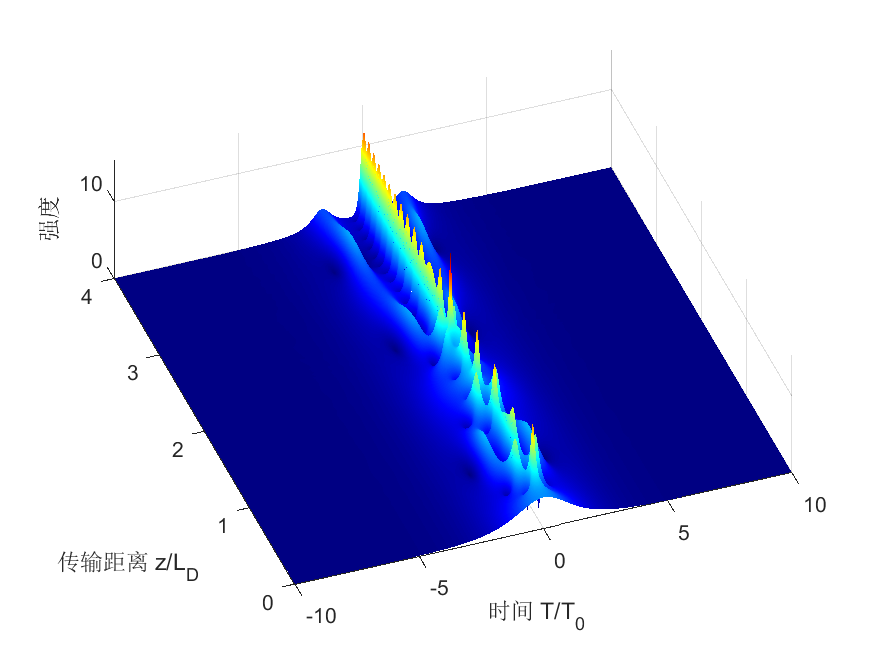
\includegraphics[width=0.45\linewidth]{FDM_四阶孤子_侧视图.png}
        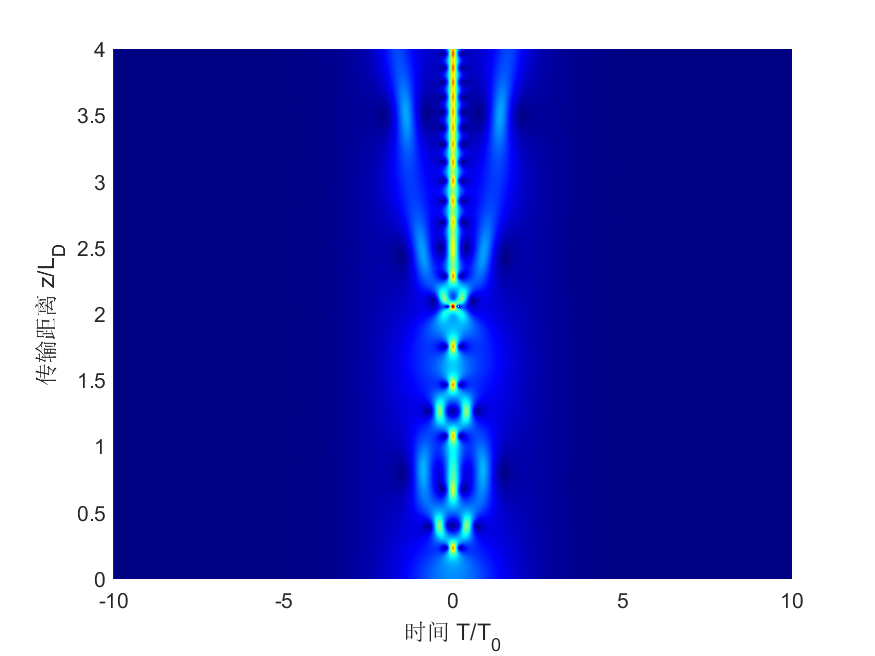
\includegraphics[width=0.45\linewidth]{FDM_四阶孤子_俯视图.png}
        \caption{$u(0,\tau)=4\mathrm{sech}(\tau)$}
        \end{minipage}
    \end{subfigure}
    \caption{有限差分模拟的孤子周期性演化}
    \label{fig:FDM}
\end{figure}